\section{Influence of pivot selection}

In this experiment we establish a baseline for selecting pivots on partition-based sorting algorithms. While it is commonly known that randomized approaches are the most effective way of dealing with unknown distributions~\cite{estivil92}, in this approach we want to confirm if by biasing the selection on the partitioning stages of the algorithms have any direct influence over its running time.\\

\subsection{Understanding pivot bias}

As explained before in Section~\ref{SECTION:PARTITIONING_SCHEMES}, all partition based algorithms are based in the idea of generating two equal sized partitions, which contributes to a continuous decrease by a factor of 2 on each iteration. Under normal circumstances, it is expected that $log_2(n)$ partition operations are executed for a given sequence of $n$ size.\\

But this assumption only yields when there is only one pivot to select. Meaning that there is a single element which divides both partitions generated by the algorithm, so for the case of a \emph{three-way-partition} it does not apply. Let us take a example of a sequence $S$ of size $n$ which contains $n$ unique integer elements. So, by induction on the integer number definition, each element if used as pivot for a partition can only yield one and only one pair of partition sets on $S$.\\

When repeated elements are found on $S$ we face a problem with the definition itself of partition presented in Section~\ref{SUBSECITON:PARTITIONING_PROBLEM}, as there is no guarantee that the partitioned element is present or not in the resulting array. Using a three-way partitioning element does not solve the problem of reducing the search space and in this regard we have the following two options:

\begin{itemize}
    \item Group the repeated elements and threat that set of repeated element as they were a unique element on $S$ --- we discuss this approach on Section~\ref{SECTION:STACK_STRUCTURE}.
    \item Preserve the elements into the array and we apply a set of rules to choose which element deliver as our pivot.
\end{itemize}

This makes a lot of sense when revisiting the plot at Figure~\ref{FIG:BENCHMARK_05_CLASSES}, as the more predominant is a certain class in a sequence, the less important becomes the pivot value selected but their final position.\\

\subsection{Effects on the partitioning}

Let us consider the pivot bias as a rational number $p_b \in [0,1]$. This bias allows us to map to indexes in $S$ to a floating point representation by assuming $S_i = \lfloor n\cdot p_{b}  \rfloor, \forall ~i~ \in[0,\norm{S}($. In colloqual terms, this means that a index of $0.0$ means that the returned pivot belongs to the leftmost index of the middle segment, a value of $0.5$ a pivot in the middle of the segment and $1.0$ the rightmost element, asumming that the elements are sorted in a ascending fashion.\\

\begin{figure}
    %BENCHMARK_06_NOISE_BIAS
    %01_basebenchmark_06_noise_bias
    \centering
    \begin{subfigure}[b]{0.45\textwidth}
        \centering
        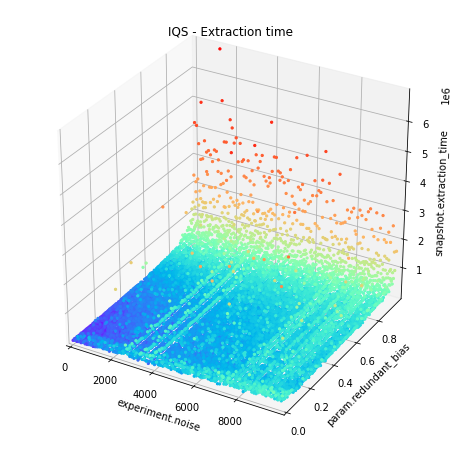
\includegraphics[width=0.9\textwidth]{./fragments/04_experimental_execution/images/01_basebenchmark_06_noise_bias.png.1_0.png}
        % 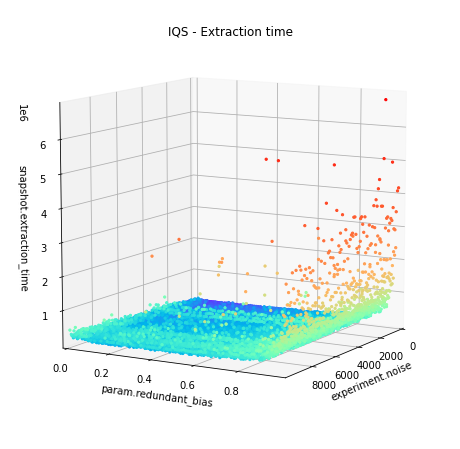
\includegraphics[width=0.40\textwidth]{./fragments/04_experimental_execution/images/01_basebenchmark_06_noise_bias.png.1_1.png}
        % \includegraphics[width=0.40\textwidth]{./fragments/04_experimental_execution/images/01_basebenchmark_06_noise_bias.png.1_2.png}
        \caption{IQS}
        \label{FIG:BENCHMARK_06_NOISE_BIAS__0_0}
    \end{subfigure}
    \hfill
    \begin{subfigure}[b]{0.45\textwidth}
        \centering
        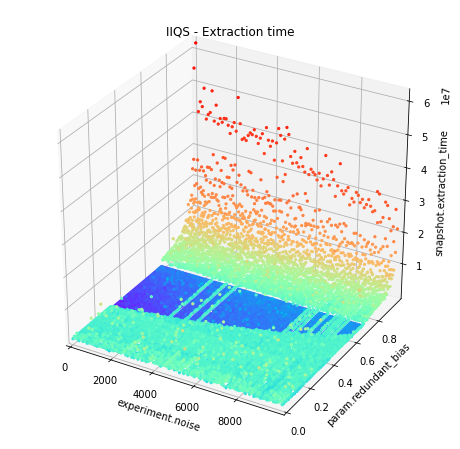
\includegraphics[width=0.9\textwidth]{./fragments/04_experimental_execution/images/01_basebenchmark_06_noise_bias.png.0_0.png}
        %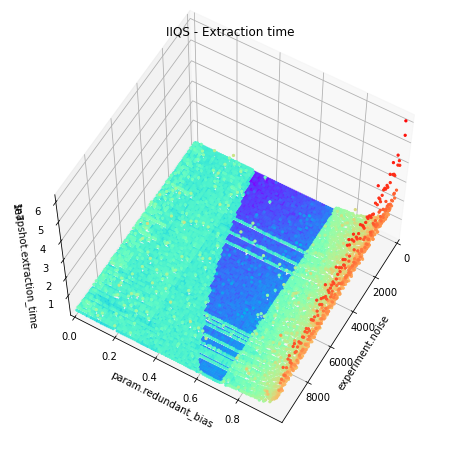
\includegraphics[width=0.40\textwidth]{./fragments/04_experimental_execution/images/01_basebenchmark_06_noise_bias.png.0_1.png}
        \caption{IIQS}
        \label{FIG:BENCHMARK_06_NOISE_BIAS__0_1}
    \end{subfigure}

    \caption{Random noise and pivot bias benchmark for random noise impact on extraction time.}
    \label{FIG:BENCHMARK_06_NOISE_BIAS}
\end{figure}

For our first observation we limit the result to only examine the first extraction performed by IQS, as it is already known that it is the most compute intensive operation in this algorithm. Then, we can observe in Figure \ref{FIG:BENCHMARK_06_NOISE_BIAS} that both the noise amount and the bias over the partition have a huge impact when extracting the first element in the sequence which is also different for both implementations of the algorithm.\\

% By examining the extra information provided by our first experiment, there are two noticeable details on the effect of biasing the selection of the resulting pivot. 
There are some interesting effects of the sequence noise for the repeating case instance. IQS shows the best performance as the noise decreases but also as the pivot bias is more inclined towards selecting the smaller elements. But this effect it is only an illusion generated by the same case depicted on Figure~\ref{FIG:BENCHMARK_02_ASC_CASE}, as less noise is found in the sequence, the greater the chance to select as pivot an element belonging to the repeating portion of the sequence, hence the bias effect studied on IQS for the partition comes into full effect. Both changing the bias towards greater values and to increase the noise contributes to increase the extraction time, it is clear that the bias has a greater effect than noise. \\

Then something interesting happens on IIQS, as the behaviour is not as smooth as on IQS case. There is a valley that it appears to be in function of the bias, which for certain amounts of noise in the sequence it favours their execution. This is because of a forced execution of the introspective steps. Both noise and pivot bias have a huge impact on the times that this step is executed, hence, aditional $O(n)$ time is consumed on the iteration when the noise exceeds IIQS fixed $\alpha$ and $\beta$ constraints~\cite{7416566}. In the same fashion as our previous observations, the fact that this effect decreases when inducing more noise is related to the probability of randomly selecting a pivot which belong to a repeated portion of the array. When this happens we notice a great reduction of the running time, which suggest that we should adjust our pivot bias to match our $\alpha$ and $\beta$ values in order to get the best performance.\\


\begin{figure}
    %BENCHMARK_07_NOISE_BIAS
    %01_basebenchmark_07_extraction_bias
    \centering
    \begin{subfigure}[b]{0.45\textwidth}
        \centering
        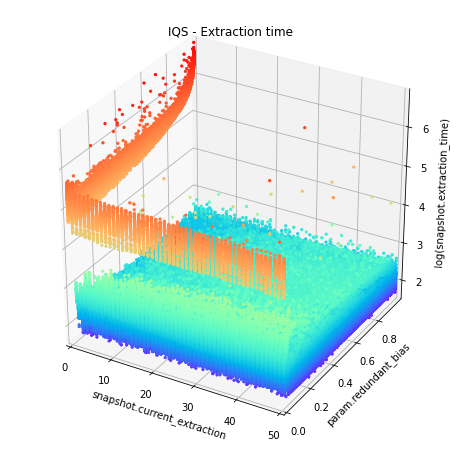
\includegraphics[width=0.9\textwidth]{./fragments/04_experimental_execution/images/01_basebenchmark_07_extraction_bias.png.1_0.png}
        % 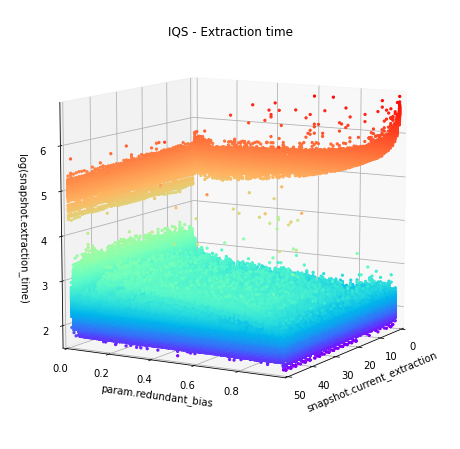
\includegraphics[width=0.40\textwidth]{./fragments/04_experimental_execution/images/01_basebenchmark_07_extraction_bias.png.1_1.png}
        % \includegraphics[width=0.40\textwidth]{./fragments/04_experimental_execution/images/01_basebenchmark_07_extraction_bias.png.1_2.png}
        \caption{IQS}
        \label{FIG:BENCHMARK_07_NOISE_BIAS__0_0}
    \end{subfigure}
    \hfill
    \begin{subfigure}[b]{0.45\textwidth}
        \centering
        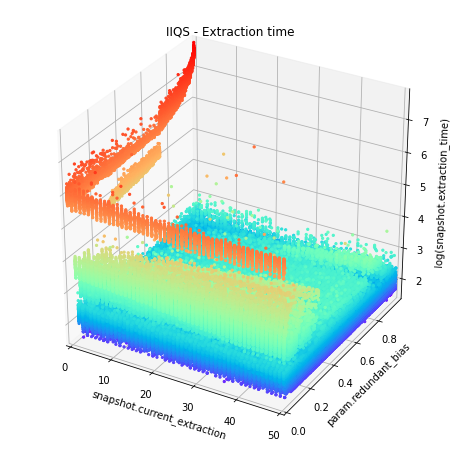
\includegraphics[width=0.9\textwidth]{./fragments/04_experimental_execution/images/01_basebenchmark_07_extraction_bias.png.0_0.png}
        %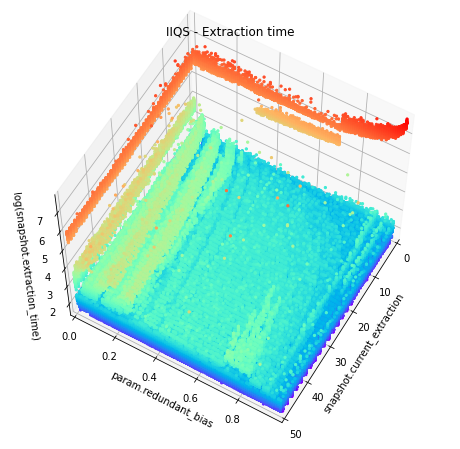
\includegraphics[width=0.40\textwidth]{./fragments/04_experimental_execution/images/01_basebenchmark_07_extraction_bias.png.0_1.png}
        \caption{IIQS}
        \label{FIG:BENCHMARK_07_NOISE_BIAS__0_1}
    \end{subfigure}

    \caption{Pivot bias and extraction benchmark impact on extraction time.}
    \label{FIG:BENCHMARK_07_NOISE_BIAS}
\end{figure}


Let us assume now that there is no noise in our sequence, in order to match a best case execution for IQS. Then by looking the effects of the pivot bias against the subsequent extractions in Figure~\ref{FIG:BENCHMARK_07_NOISE_BIAS} we notice setting our pivot bias towards the leftmost elements in the pivot segment is not a good idea. When there is only one class and there is no noise in the sequence, the extractions become more costly as the pivot bias deviates from the ideal $0.5$ value. This holds for both the first extraction and the subsequent ones. Also, it does clearly state that fixing the pivot bias to one extreme or another is not a good idea. \\

For IIQS the same rules apply, with the difference that there is a boost of performance when the bias belongs to the $[\alpha,\beta]$ range, as the introspective step rearranges the element and this ends being more cheaper in some cases than to continue the partition stage blindfolded.\\

\FloatBarrier